\documentclass[12pt,a4paper,oneside]{book}

\usepackage{graphicx} % Required for inserting images
\usepackage{hyperref}
\usepackage{babel}
\usepackage{xeCJK}
\usepackage{parskip}
\usepackage{caption}
\usepackage{setspace}
\usepackage{fontspec}
\usepackage{minted}
\usepackage{xcolor}
\usepackage{longtable}
\usepackage{geometry}
\usepackage{lscape}
\usepackage{tabularx}
\usepackage{appendix}
\usepackage{fancyhdr}
\usepackage[acronym, nonumberlist]{glossaries}

\makeglossaries
\glsdisablehyper
\newacronym{bleu}{BLEU}{Bilingual Evaluation Understudy}
\newacronym{rouge}{ROUGE}{Recall-Oriented Understudy for Gisting Evaluation}
\newacronym{bp}{BP}{Brevity Penalty}
\newacronym{pngram}{pn\_gram}{Precision score for a specific n-gram length}
\newacronym{lcs}{LCS}{Longest Common Subsequence}
\newacronym{mt}{MT}{Machine Translation}
\newacronym{alpac}{ALPAC}{Automatic Language Processing Advisory Committee}
\newacronym{nmt}{NMT}{Neural Machine Translation}
\newacronym{smt}{SMT}{Statistical Machine Translation}
\newacronym{ipc}{IPC}{Indian Penal Code}
\newacronym{nlp}{NLP}{Natural Language Processing}
\newacronym{nltk}{NLTK}{Natural Language Toolkit}
\newacronym{csv}{CSV}{Comma-Separated Values}
\newacronym{llm}{LLM}{Large Language Model}
\newacronym{sl}{SL}{Source Language}
\newacronym{tl}{TL}{Target Language}
\newacronym{st}{ST}{Source Text}
\newacronym{tt}{TT}{Target Text}
\newacronym{rbmt}{RBMT}{Rule-Based Machine Translation}
\newacronym{ebmt}{EBMT}{Example-Based Machine Translation}
\newacronym{bert}{BERT}{Bidirectional Encoder Representation from Transformers}
\newacronym{gpt}{GPT}{Generative Pre-trained Transformers}


\pagestyle{fancy}
\renewcommand{\headrulewidth}{0pt}
\fancyhead[R]{}

\newfontfamily\hindifont{Noto Sans Devanagari}[Script=Devanagari]

\setlength{\parskip}{8pt}
\setlength{\parindent}{16pt}
\doublespacing

\begin{document}
\frontmatter

\begin{titlepage}
\singlespacing
\begin{center}
\Large
\textbf{Machine Translation: Developments \& Issues, with Special Reference to IPC}
\small
\vspace{1cm}

A dissertation submitted for the fulfillment of the degree of
\\\textbf{Integrated MSc. in Linguistics and Language Sciences}

\vspace{1cm}


\includegraphics[width=4.5cm]{images/curaj.png}

\vspace{1cm}

Submitted By

\vspace{0.1cm}

\textbf{Bhanu Pratap Singh}\\
Int. MSc. in Linguistics and Language Sciences (2019-2024)\\
2019IMSLI003

\vspace{1cm}

Supervisor

\vspace{0.1cm}

\textbf{Dr. Dhananjay Kumar Tiwari}\\
Assistant Professor\\
Department of Linguistics\\
Central University of Rajasthan

\vspace{1cm}

\textbf{Department of Linguistics\\
School of Humanities \& Languages\\
Central University of Rajasthan\\
2024
}

\end{center}
\doublespacing
\end{titlepage}

\clearpage
\begin{center}
\textbf{
    Central University of Rajasthan\\
    Department of Linguistics\\
    School of Humanities and Languages\\
    }
    \vspace{2cm}
\textbf{\large DECLARATION}
\end{center}

\noindent

\rightline{27 May 2024}

\vspace{0.5cm}
\onehalfspacing
I declare that the dissertation titled -``Machine Translation: Developments and Issues, with Special Reference to IPC” is a record of bonafide research that I have conducted under the supervision of Dr. Dhananjay Kumar Tiwari, Assistant Professor at the Department of Linguistics, for the partial fulfillment of the Degree Int. MSc. in Linguistics and Language Sciences. This Dissertation is an original piece of research, and no part of this work has been submitted for the award of any degree or diploma of this University or any other University.

\vspace{5cm}

\rightline{Bhanu Pratap Singh}
\rightline{Int. MSc. Linguistics and Language Sciences}
\rightline{2019IMSLI003}
\rightline{Department of Linguistics}
\rightline{Central Univeristy of Rajasthan}
\doublespacing

\clearpage

\clearpage

\begin{center}
\textbf{
    Central University of Rajasthan\\
    Department of Linguistics\\
    School of Humanities and Languages\\
    }
    \vspace{2cm}
\textbf{\large CERTIFICATE}
\end{center}

\noindent

\rightline{27 May 2024}

\vspace{0.5cm}
\onehalfspacing

This is to certify that the dissertation titled -``Machine Translation: Developments and Issues, with Special Reference to IPC” submitted by Bhanu Pratap Singh, bearing Enrollment Number 2019IMSLI003, of the Department of Linguistics, School of Humanities and Languages, for the award of the degree of Int. MSc. in Linguistics and Language Sciences is bonafide research carried out by him under my supervision. The contents of this Dissertation, in full or in parts, have not been submitted for the award of any degree or diploma of this University or any other Institute or University.

\vspace{2cm}

\rightline{Dr. Dhananjay Kumar Tiwari}
\rightline{Assistant Professor}
\rightline{Department of Linguistics}

\noindent\rule{\linewidth}{0.1pt}
\noindent
This dissertation may be placed before the external examiner for final evaluation.

\vspace{2cm}

\rightline{Head$\backslash$Coordinator of the Department}
\rightline{Department of Linguistics}

\doublespacing
\clearpage


\clearpage

\begin{center}
    \textbf{\Large Acknowledgement}
\end{center}

\vspace{1cm}
\onehalfspacing
\noindent

I would like to express my sincere gratitude to every individual whose support and guidance have been invaluable throughout the completion of this thesis.

First and foremost, I am deeply grateful to my supervisor, Dr. Dhanajay Kumar Tiwari, for his unwavering support, insightful guidance, and constant encouragement. His expertise and feedback have been crucial in shaping this thesis.

I am also thankful to my friends Keshav, Siddharth, Sandeep, Chetna, Dharm, and many others, whose support, discussions, and encouragement have been immensely helpful throughout this journey. Their assistance and companionship have made this challenging process more manageable and enjoyable.

I would also like to extend my gratitude to all the faculty members of the Department of Linguistics, for their support, feedback, and suggestions.

A special mention goes to the late William John Hutchins, whose pioneering work and extensive research in the field of machine translation have been a cornerstone for my thesis. His compilations and summaries on the development of machine translation since its inception have provided a substantial foundation and inspiration for my research.

Finally, I would like to thank my family for their continuous support and understanding during my studies. Their belief in me has been a driving force in my academic pursuits.

Thank you all for your invaluable support.

\vspace{2cm}
\rightline{Bhanu Pratap Singh}
\rightline{2019IMSLI003}
\doublespacing

\clearpage

\clearpage

\vfill
\begin{center}
    \textbf{\Large Abstract}
\end{center}

\vspace{1cm}

\noindent

\textit{This thesis explores the advancements and challenges in the field of machine translation, with a specific focus on translating legal texts within the Indian Penal Code (IPC). The study evaluates two prominent neural machine translation (NMT) systems, Google Translate and Azure Translate, comparing their performance in translating Hindi IPC sections into English. Data was collected from official legislative sources and processed using Python on Google Colab, with translations assessed through both automated metrics (BLEU and ROUGE scores) and human evaluation. The results highlight the strengths and weaknesses of each system, offering insights into the efficacy of current NMT technologies in handling complex legal language. The findings underscore the importance of continuous development in machine translation to improve accuracy and fluency, particularly for resource-scarce languages and syntactically diverse language pairs.}
\vfill
\clearpage

\listoffigures
\listoftables

\singlespacing
\printglossary[type=\acronymtype, title=List of Abbreviations]
\doublespacing


\mainmatter

\tableofcontents

\phantomsection
\chapter{Introduction}

There are many unanswered questions about the mysteries of the mind and brain. One of the major mysteries, and also one of the primary characteristics of us as humans, is Language. By Language here we do not mean the specific instances such as English, Hindi, German, etc. but rather the general ability of Language. This ability enables us to convey the most abstract ideas that our minds can create, in the form of strings of arbitrary sounds or signs, as well as to decode and receive the said information and ideas from these strings of arbitrary sounds or signs.

From this perspective, we could define Language as an information encoding system \cite{coupe2019different}, through which we encode our thoughts into strings of speech sounds or signs to communicate these thoughts to others. To reiterate, information in our mind is encoded (or in a manner - translated) into a string of speech sounds or signs, which after going through a medium is received by the recipient, who then decodes these sequence of speech sounds or signs, receiving the information to be conveyed, thus completing the process of communication \cite{shannon1948mathematical}.

\begin{figure}[h]
    \centering
    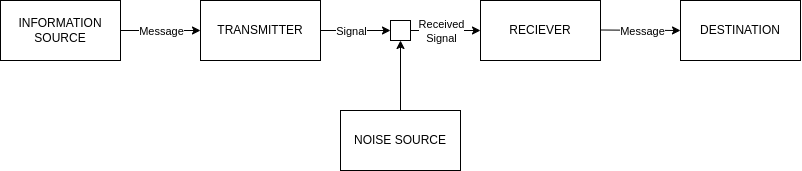
\includegraphics[width=0.96\textwidth]{images/InformationProcess.drawio.png}
    \caption{Shannon's model of the process of communication}
\end{figure}

Translation may be seen as another step added to this process. Information encoded in one language (\gls{sl}) is to be transferred into an utterance in another language (\gls{tl}). In a way, the nature of the process of translation is similar to that of the nature of Language itself, both are trying to maintain the integrity of meaning/information changing from one form to another. Well, even that is an oversimplification of the idea of translation and the phenomenon of language.

\phantomsection
\section{Translation}

 The human experience thrives on stories, ideas, and emotions, all intricately woven with the threads of language. Yet, the very beauty of language lies in its diversity, a vibrant tapestry of tongues that both connects and separates us. Language is one yet languages are many, this distinction and the necessity to bridge this gap is why we need translation \cite{ricoeur2007translation}. Translation is far from a simple act of word substitution. It's a labyrinthine journey, a constant negotiation between being faithful to the source text and the need to create a work that resonates with the target audience, while also being mindful of the socio-cultural contexts of this bilateral exchange.
 
Many theorists have presented their definition of translation focusing on various paradigms. Catford for one defines translation as ``{\itshape the replacement of textual material in one language (\gls{sl}) by equivalent textual material in another language (\gls{tl}).}", this approach draws upon a theory of language, a general linguistic theory \cite{catford1965linguistic}. In this definition, the focus is on meticulously replacing textual material in the source language with its closest counterpart in the target language. Imagine a meticulous puzzle, where each piece from the source language must find its perfect fit in the target language, ensuring accuracy in the transfer of information. This approach prioritizes faithfulness to the literal meaning of the text, relying on established linguistic theories for guidance.
 
 Nida presents a different view emphasizing the message involved in this exchange, he proposes the idea of dynamic equivalence and defines translation as - ``{\itshape the closest natural equivalent of the source-language message, first in terms of meaning and secondly in terms of style}" \cite{nida1964toward} \cite{jixing2013translation}. The aim is to create a text in the target language that resonates with the new audience in the same way the original resonated with its intended readers, by capturing not just the raw meaning of the words, but also the stylistic nuances, the emotional weight, and the cultural references embedded within the original work.

 The complexity involved in the translation process is observed, endowing it with the characteristics of both an art and a science \cite{nida1964toward} \cite{bell2016translation}.

\phantomsection
\section{Machine Translation}

Commerce and war have been a major driving force behind several technological advances, which also include translation. Translation is a necessity when it comes to the interaction and trade beyond geographical boundaries. Even though geograp-hical limitations have been somewhat overcome, bringing people closer in the vast virtual world, the problem of communication stands, and so does the necessity of translation \cite{bhattacharyya2015machine}. 

\gls{mt} was brought into serious consideration in the 1950s with the advent of modern computers. It was the first computer-based application of \gls{nlp} \cite{hutchins1992introduction}. Since then the progress of Machine Translation has not exactly been linear. The \gls{alpac} report of 1966 dealt a heavy blow to the development of Machine Translation, nearly halting more of the developments in this field \cite{poibeau20171966}. Yet the developments did not completely stop, and \gls{mt} has since come a long way. Though it has not achieved human-level accuracy \cite{rivera2022machine}, it still produces astonishing results.

\gls{mt} has seen a lot of developments in the past few decades. Providing an overview of these developments is one of the objectives of this work, especially highlighting the progress made in the last two decades, especially in the context of \gls{nmt}. Although modern machine translation approaches are mostly data-driven, there have been other approaches whose impact is still prevalent.

\gls{rbmt} and Data-Driven or Corpus-Based MT are two major approaches under which most of the techniques for Machine Translation fall \cite{bhattacharyya2015machine}. RMBT techniques were the first approach adopted; some of the techniques involved were direct approach, involving the use of bilingual dictionaries and morphological analysis to translate the source text word by word without much focus on the syntactic nuances of the SL or TL.  Transfer-based and Interlingua MT, in which the attempt is to convert the Source Text into an intermediate representation, a formal one for transfer-based techniques, and an abstract one for Interlingua, which is then converted to the Target Language Text \cite{baker2019routledge}.

The advent of the information age and the increase in both computing power and availability of large corpora lead to the development of data-driven/corpora-based MT techniques. \gls{smt} and \gls{ebmt} are the outcomes of these developments \\ \cite{baker2019routledge}. SMT learns from a massive collection of bilingual texts to translate languages. It uses a "translation model" to find the most likely translations of words and phrases, and a "language model" to ensure that the translated sentences are grammatically correct \cite{hutchins2006future}. However, EBMT works like a giant library of translated examples. When given a new text to translate, EBMT searches this library for the closest existing translations (matching). Then it identifies the relevant parts from those translations (alignment) and recombines them to fit the new text grammatically (recombination).


\phantomsection
\subsection{Neural Machine Translation}

Leveraging modern high-performance computing and massive amounts of data, has allowed a new technology for Machine Learning to take form, i.e. Artificial Neural Networks, especially Deep Neural Networks. The application of this technology in translation has given rise to a new approach - Neural Machine Translation (NMT). The work has been going on for quite a while, for example, Robert B. Allen's demonstration of the use of a feed-forward neural network to translate from English to Spanish with a vocabulary length of 31 \cite{allen1987several}.

\begin{figure}[h]
    \centering
    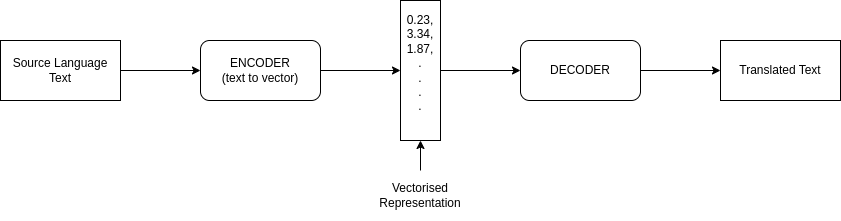
\includegraphics[width=0.96\textwidth]{images/EncoderDecoder.png}
    \caption{Encoder-Decoder Architecture}
    \label{fig:encode-decode}
\end{figure}

A major breakthrough in this approach was made in 2013-14, with the use of Convolutional Neural Networks (CNNs) and Recurrent Neural Networks (RNNs) to encode SL text into an intermediate representation, which was then decoded using an RNN-based decoder for TL \cite{kalchbrenner2013recurrent} \\ \cite{cho2014learning} \cite{sutskever2014sequence}. There were limitations to this approach, i.e., they faced difficulties when dealing with longer sentences, which was addressed with the introduction of {\itshape Attention} \cite{bahdanau2014neural}. Attention was an important component that led to the development of Large Language Models (LLMs).

Google in 2016 released a massive NMT system, which performed quite well, making NMT a go-to research area for most of the translation research since then \cite{wu2016google}. In 2017 came the paper titled "Attention is all you need" \cite{vaswani2017attention} which revolutionized Artificial Intelligence, giving rise to massive Multi-modal Large Language Models, enabling various technologies to take shape, especially language technologies. Though most of the NMT systems today are sequence-to-sequence models, they have become much more powerful and effective.

\phantomsection
\section{Legal Translation}

The importance of language in law is an indisputable fact. Just like any other form of human communication and affairs, human law cannot exist without language, but language is a complicated matter. It enables us to tell truths, lies, truths that seem like lies, and lies that seem like truth. Ambiguity in law is a fatal flaw, and ambiguity, more often than not has the potential to turn up in language use.

Legal language needs to be very particular and accurate, this presents a very peculiar problem for translators, where they not only have to focus on finding an equivalence for the message but also preserve its structure integrity in a disambiguate manner.

In modern times where numerous tasks have been handed over to machines, especially translation, and it's application for legal translation isn't too far off. The use of Machine Translation in a legal context will become prevalent, but to what extent is yet to be seen. One must be very careful with such sensitive matters as \cite{deborah2023challenges} exemplifies - 

\begin{quote}
Translation, especially in legal contexts, can carry significant consequen-ces. After all, one may never know whether the translation of the Chinese word 夷 \textit{yi} or 蛮夷 \textit{manyi} as ‘barbarians’ or ‘foreign barbarians’, as opposed to ‘foreigners’, contributed to the start of the Opium Wars (1839–1860) between China and Western countries all those years ago.
\end{quote}

As we must have all experienced, this kind of error is one of the prevalent flaws of many MT systems. Thus, the use of MT for a sensitive application such as legal translation must be done under numerous considerations.

\phantomsection
\section{Indian Penal Code}

The \gls{ipc}, while no longer in use, is an extremely important document in India's legal history, and defined India's criminal code for over one and a half centuries, until recently, when it was replaced by Bharatiya Nyaya Sanhita in December 2023. 

Drafted in 1860 by the British Raj, it aimed to be a unified code covering all major crimes \cite{devadas2016history}. It outlines various offenses, from theft and assault to murder and treason. It also established a system of punishments, including imprisonment, fines, and even the death penalty. The code aimed to be clear and concise, ensuring everyone understood what constituted a crime and its corresponding consequences.

The IPC was broadly categorized into four parts. The initial chapters (I-V) laid the groundwork, defining legal terms and establishing principles of liability. Chapters VI-XV then addressed offenses impacting the state, public order, and safety. Chapters XVI-XXII formed the core, encompassing crimes between individ-uals like theft, assault, and property damage. Finally, Chapter XXIII served as a safety net for uncategorized attempts to commit crimes \cite{devadas2016history}.

Let's look at an excerpt from IPC, Chapter VIII - Section 144:-

\begin{quote}
    \emph{\textbf{English}} \\ \textbf{Joining unlawful assembly armed with deadly weapon} — Whoever, being armed with any deadly weapon, or with anything which, used as a weapon of offense, is likely to cause death, is a member of an unlawful assembly, shall be punished with imprisonment of either description for a term which may extend to two years, or with fine, or with both.
\end{quote}

\begin{quote}
\emph{\textbf{{\hindifont हिंदी}}} \\
 \textbf{{\hindifont घातक आयुध से सज्जित होकर विधिविरुद्ध जमाव में सम्मिलित होना}} -  {\hindifont जो कोई किसी घातक आयुध से, या किसी ऐसी चीज से, जिससे आक्रामण आयुध के रुप में उपयोग कये जाने पर मृत्र्यु कारित होनी सम्भाव्य है, सज्जित होते हुए किसी विधिविरुद्ध जमाव का सदस्य होगा, वह दोनों में से किसी भांति के कारावास से, जिसकी अवधि दो वर्ष तक की हो सकेगी, या जुर्माने से या दोनों से, दण्डित किया जायेग। }
\end{quote}


\phantomsection
\section{Theoretical Framework: Dorr's Divergence}

Bonnie J. Dorr, in her paper titled "Machine Translation Divergences: A Formal Description and Proposed Solution" \cite{dorr1994machine}, talks about various issues which come up when a translation task is taken up, these issues are termed as translation divergences, these divergences are essentially cross linguistic differences which make the direct linear transfer from SL to TL impractical. She presents solutions to these divergences in her paper, which are derived from the formalization of two types of information - (1) the linguistically grounded classes upon which lexical-semantic divergences are based; and (2) the techniques by which lexical-semantic divergences are resolved. Let us take a look at some of the divergences proposed by Dorr.

\paragraph{Thematic Divergence}

Thematic Divergence involves the repositioning of the arguments with respects to a head, a change in the thematic role of the argument. This type of divergence arises only in cases in which there is a logical subject present.

\begin{quote}
English: I like Mary \\
Spanish: Maria me gusta a mi (Mary pleases me)    
\end{quote}

\paragraph{Promotional Divergence}

Promotional Divergence connotes the promotion of logical modifier into a main verb position, i.e. logical modifier becomes the syntactic head and the syntactic head becomes an internal argument.

\begin{quote}
English: John usually goes home \\
Spanish: Juan suele ir a casa (John tends to go home)
\end{quote}

\paragraph{Demotional Divergence}

Demotional Divergence is the opposite of Promotional Divergence, i.e., logical head gets associated with syntactic adjunct position and logical argument is associated with syntactic head position.

\begin{quote}
English: I like eating \\
German: Ich esse gern (I eat likingly)
\end{quote}

\paragraph{Structural Divergence}

Structural Divergence results in change of the syntactic class associated with a syntactic constituent.

\begin{quote}
English: John entered the house \\
Spanish: Juan entro en la casa (John entered the house)
\end{quote}

\paragraph{Conflational Divergence}

Conflational Divergence occurs when sense of one word in SL is described by more than one word in TL.

\begin{quote}
English: I stabbed John \\
Spanish: Yo le di punaladas a Juan (I gave knife-wounds to John)
\end{quote}

\paragraph{Categorical Divergence}

Categorical Divergence happens when part-of-speech (POS) property of a word/constituent in SL changes during translation to TL.

\begin{quote}
English: I am hungry \\
German: Ich habe hunger (I have hunger)
\end{quote}

\paragraph{Lexical Divergence}

Lexical Divergence happens when there is no exact equivalent of a word/constituent in SL in TL, thus some other word/constituent is used to express a sense which is somewhat similar to the original sense.

\begin{quote}
English: John broke into the room \\
Spanish: Juan forzo la entrada al cuarto (John forced (the) entry to the room)
\end{quote}

There are several other types of divergences as discussed by Dorr. These divergences are an important basis for judging machine translation systems.

\phantomsection
\section{Motivation for Research}

For our course in Semester IX, concerned with computational linguistics, we had to analyze the systematic divergences observed in translating short stories from Hindi to English. Though the translation was more often than not, acceptable, there was still situations where the divergences posed were severe and caused a major loss of sense in the process of translation. This may be fine in the case of non-consequential texts like a short story, but in the case of things like legal texts, contracts, and judgments, minor cases of linguistic ambiguity, let alone such major divergences have major consequences. Thus, with the aim to analyze the development and systematic performance of these tools, I took up this study. 

\phantomsection
\section{Problem Identification}

As highlighted, even though MT has come a long way, it is still far from perfect. There are still several sets of issues present. For resource-rich languages such as English, German, etc. this set of issues is small, but for languages lacking resources and also for language pairs with a wide difference between their syntactic and morphological structures, this set is still large. Issues like lexical divergence, syntactic divergence, improper cognate transfer, and artificiality are still present, and in the case of legal translation, these kinds of divergences might present serious issues. 

English is the most resource-rich language, and Hindi could be said to have the largest speaker base in India. Translation between these two languages should be relatively better, compared to a language pair such as Japanese and Santali. But how accurate would it be in terms of accuracy, and how the issues observed would create problems for translating legal text is what we wished to explore in this study, while also appreciating how far the field of Machine Translation has come.

\phantomsection
\section{Research Questions}

\begin{itemize}
    \item How has Machine Translation developed over the decades?
    \item What is the performance of modern Machine Translation tools?
\end{itemize}

\phantomsection
\section{Objectives}

\begin{itemize}
    \item To summarize the development of Machine Translation over the decades.
    \item To evaluate the effectiveness of Machine Translation tools, with a focus on legal translation.
\end{itemize}

\phantomsection
\section{Limitations}

For this study took a sample of the 511 Sections of the IPC in Hindi, and translate them into English by using two NMT tools - Google Translate and Azure Translate. After translating we analyzed the translation. We used automated metrics, as well as human evaluation. The details of the sampling, analysis, the metrics, and the tools used are discussed in detail in Chapter \ref{chap:meth}.

The metrics we used for this study are BLEU and ROUGE, both of these approaches require multiple reference translations to perform well, but in the case of this study, we have been only able to provide one reference translation. Also, only one human participant was employed to score the translations. However, these limitations do not have that great of an influence on the result of this study, as we do get a rough picture of where these translation tools stand.

\phantomsection
\chapter{Developments in Machine Translation - Overview}

Machine Translation has a relatively brief history, comparable to that of modern computer science. It is the earliest application of Natural Language Processing using modern computers, that was conceived in the 1950s. However, the idea of using machines to assist translation isn't something new; The use of mechanical dictionaries in translation was first suggested in the 17th century\\ \cite{hutchins1992introduction}, and the techniques used for translation which are incorporated to produce a mechanized model of translation are even older, tracing back to 9th-century Arabic scholar named \textit{Al-Kindi}. His statistical observations and techniques for systematic translation produced results that even affected other domains of Computational Linguistics, such as authorship analysis and stylometrics \cite{dupont2018cryptological}.

In 1930, two patents were applied for mechanical bilingual dictionaries, one by French-Armenian Georges Artsrouni and another by a Russian Petr Troyanskii \cite{hutchins2001machine}. The latter held more importance as it proposed not only a method for a bilingual dictionary but also coding and interpreting grammatical functions using `universal' Esperanto-based symbols \cite{hutchins2005history}. However, the notion of using modern computers for translation originated from the depth of another research - cryptography. 

\phantomsection
\section{Cryptography, Translation \& Weaver}

Machine Translation was for a long time treated as a problem of cryptology \cite{dupont2018cryptological}. The origin of modern idea of the use of computers for Machine Translation can be traced back to Warren Weaver. In his discussions with Norbert Wiener, he presents his observations regarding the systematic encryption of language utterances into numbers using cryptographic techniques, which can then systematic-ally be decoded and return approximately the same original utterance, even if decoded by a person who doesn't know the language, as observed in cryptography \\ \cite{locke1954mechanical}. His perspective could be surmised by an excerpt from his letters to Wiener -

\begin{quote}
    One naturally wonders if the problem of translation could conceivably be treated as a problem in cryptography. When I look at an article in Russian, I say: `This is really written in English, but it has been coded in some strange symbols. I will now proceed to decode.'
\end{quote}

It was in his memorandum titled `Translation' in July 1949, that Weaver proposed his ideas, and presented his views on Machine Translation and the use of computers, statistics, and even neural networks for the purpose of translation \cite{hutchins1999warren}. This eventually became the driving force behind MT research in the 1950s, and its effects can be seen to date.

The memorandum first discussed the ongoing works and the progress made in the field. He put forward four proposals for further research in this field \cite{hutchins1999warren}.

\paragraph{Use of Context to Deal With Multiple Meanings} This idea could be surmised from -

\begin{quote}
    If one examines the words in a book, one at a time through an opaque mask with a hole in it one word wide, then it is obviously impossible to determine, one at a time, the meaning of words. ``Fast" may mean ``rapid"; or it may mean ``motionless"; and there is no way of telling which. But, if one lengthens the slit in the opaque mask, until one can see not only the central word in question but also say N words on either side, then, if N is large enough one can unambiguously decide the meaning. \cite{hutchins1999warren} \cite{weaver1952translation}
\end{quote}

\paragraph{Logical Elements in Language} In this proposal he brought attention to the research on mathematical modeling of neural structures of the human brain, and the use of such models in the form of robots or computers could be used to deduce any legitimate conclusion from a finite set of premises. This was under the assumption that there are logical elements in language \cite{weaver1952translation}.

\paragraph{Application of Cryptographical Methods} As discussed previously, Weaver put a lot of focus on the correlation between cryptography and translation, these ideas were primarily based on Information Theory, and the work he did with Claude Shannon \cite{hutchins1999warren}. He states -

\begin{quote}
    Frequencies of letters, letter combinations, intervals between letters and letter combinations, letter patterns, etc. which are to some significant degree independent of the language used.
\end{quote}

\paragraph{Linguistic Universals and Common Foundation for Languages} He pres-ented the notion that just like the presence of common logical features among languages, there might also by linguistics universals. In his analogy, he treats languages as towers with common basements, and that to communicate between languages one might need to descend to this common basement, i.e. the base of human communication derived by the extraction of logical features and identification of linguistic universals.

\cite{hutchins1999warren} notes that, in long term the most significant outcome of Weaver's memorandum was the appointment of logician Yehoshua Bar-Hillel to a research position at MIT (Massachusetts Institute of Technology) in 1951, which eventually led to the convening of the first conference in Machine Translation.

\phantomsection
\section{The First Generation}

The first MT conference produced great outcomes, where different scholars, discussed the direction of future research. Some of the highlights of the conference included the proposals for dealing with syntax by Oswald the Bar-Hilel, presenting arguments for a sublanguage system specifically for the purpose of translation \cite{hutchins1995machine}. 

The outcome of the conference made it obvious, that fully automatic translation would not be achievable without long-term basic research, and that in the meantime human assistance was needed for pre-editing and post-editing, i.e., preparing the SL text for translation and editing the output result to receive acceptable transla-tions \cite{reifler1952first}. There was also a discussion on the idea of a fulcrum language, a language as a point of leverage, to which and from other languages can be translated, which was discussed to be English \cite{reifler1952first}. The first requirement that numerous participants considered was a demonstration of the feasibility of Machine Translation \cite{hutchins1995machine}.

This was achieved with the Georgetown-IBM \cite{hutchins2004georgetown} experiment system in 1954, though the system was not one with practical feasibility, with only a sample of 49 carefully selected Russian sentences translated to English, with a vocabulary of only 250 words, using just 6 grammatical rules \cite{hutchins1995machine}. Yet, it achieved what it was meant to, to stimulate interest and garner large-scale funding. This also led to the rise of interest in MT in USSR \cite{hutchins1995machine}.

The research that followed either a trial-and-error based statistical approach to produce working systems (\textit{brute-force}), or a long-term solution-based theoretical approach, investing in fundamental linguistic research (\textit{perfectionist}) \cite{hutchins1995machine}. There was several works going on under different institutions in USA, as well as around the world. This was the time of Rule-Based Machine Translation. Well-known approaches were developed, `direct translation' which focuses on translation from a specific SL to a specific TL with a minimal amount of analysis and syntactic processing, `interlingua' approach, which focuses on an intermediate language independent representation. There was the `transfer approach' using 3 stages analysis, transfer, and synthesis \cite{hutchins2023machine}. Down below we have the 1985 version of the Vauquois triangle \cite{vauquois1968survey}, illustrating possible approaches in MT.

\begin{figure}[h]
    \centering
    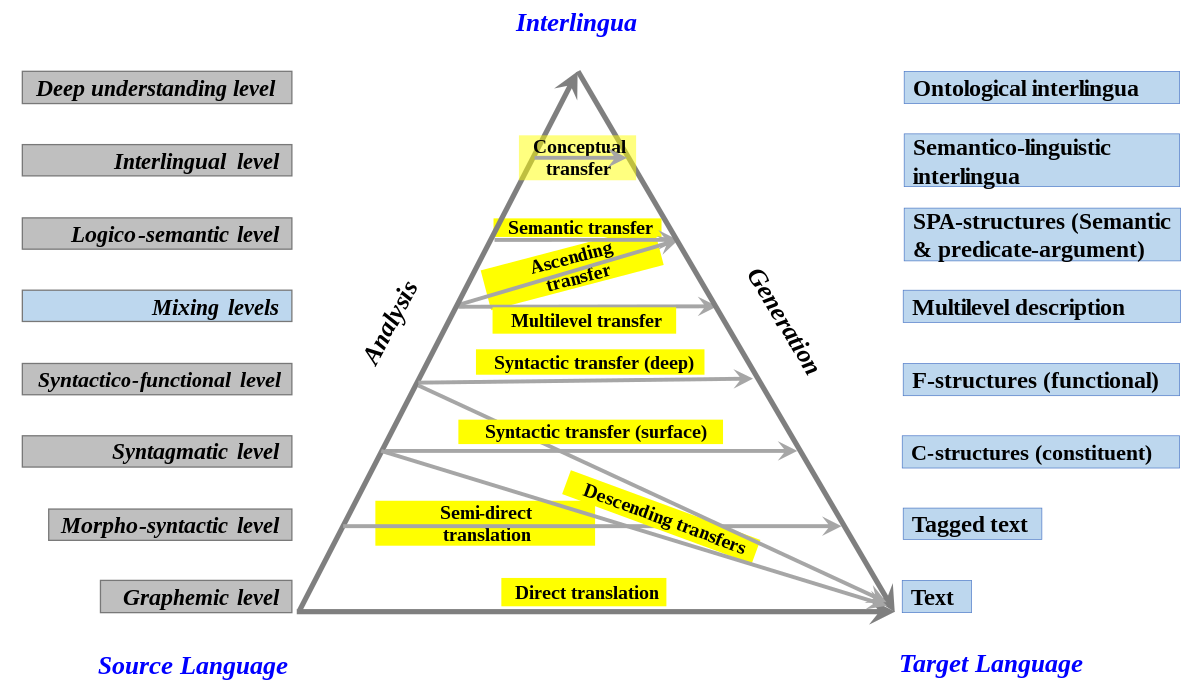
\includegraphics[width=\textwidth]{images/VauquoisModel.png}
    \caption{Vauquois triangle representing various MT approaches}
\end{figure}

Most of the research in MT, due to various reasons, hit a wall. With several institutions pulling out from the MT research altogether \cite{hutchins2023machine}, and the progress being too slow, it became a concern for the people putting in the funds.

\phantomsection
\section{ALPAC Report 1966 \& it's aftermath}

The US government sponsors becoming increasingly concerned about the lack of progress in Machine Translation, formed the Automatic Language Processing Advisory Committee (ALPAC) in 1964, which presented its first report in 1966. The report concluded that Machine Translation was twice as expensive as human translation, whereas slower, and less accurate, and that there was no predictable prospect for a useful machine translation system. It recommended that the focus be shifted to developing machine aids for human translators, such as mechanical bilingual dictionaries and other fundamental research in Computational Linguistics \cite{hutchins2023machine}. It saw no need to fund further MT research.

It had a great impact on the development of MT throughout the world, practically stagnating research in the United States for years. However, the research did not completely stop. Machine translation research just shifted direction. The new focus shifted to ``indirect" models: `interlingua' (translate text into a neutral intermediate language before converting it to the target language) and `transfer' based (analyze source and target languages separately, then transfer information for generation) \cite{hutchins2023machine}.

Examples of research projects in the 1970s and 1980s include the TAUM project (Montreal), which was successful with a syntactic transfer system for weather forecasts but struggled with complex phrases in other domains \cite{hutchins1995machine}. Another example is the ITS system (Brigham Young), which was abandoned due to complexity after a decade of development. A key trend in the 1980s was the emphasis on advanced methods and specific domains. Interlingua and transfer-based approaches continued to be explored alongside knowledge-based systems \cite{hutchins2023machine}. 

Research projects also expanded beyond North America, Western Europe, and Japan. The rise of operational machine translation systems included mainframe systems like Systran and microcomputer-based systems offered by companies like ALPS and Globalink \cite{hutchins1995machine}.

The interlingua approach faced challenges with rigidity and information loss. However, there was a renewed interest in the late 1980s with projects like DLT (Netherlands) and Rosetta (Netherlands). The transfer-based approach had influe-ntial projects like the GETA-Ariane system (Grenoble), which served as a model for many projects in the 1980s. Other notable projects included Mu (Kyoto University), SUSY (Saarbrücken), and Eurotra (European Communities) \\ \cite{hutchins2023machine}.

Knowledge-based approaches gained traction with projects in Japan, Europe, and North America. Overall, machine translation research diversified after the ALPAC report. The focus shifted to indirect models with an emphasis on practical applications. The 1980s also saw the rise of operational machine translation systems, along with the beginnings of speech translation research \cite{hutchins2023machine}.

\phantomsection
\section{Rise of Corpus-Based MT}

Till late 1980s, the field of Machine Translation was primarily dominated by the RBMT approaches, be it knowledge-based systems, or linguistics based. However, this dominance was broken in 1989, with the emergence of corpus-based methods. It began with the Candide project at IMB, which revived the long-forgotten statistics-based approach, which was suggested by Weaver and was one of the earlier approaches studied \cite{yang2014statistical} \cite{hutchins2023machine}. 

The Candide system was tested on a large corpus of French and English texts contained in the reports of Canadian parliamentary debates. The results were surprising, nearly half the translated phrases matched the exact translation present in the corpus or resulted in translations with words that presented the same sense, or any other acceptable translations \cite{berger1994candide} \cite{hutchins2023machine}.

\phantomsection
\paragraph{Statistical Machine Translation (SMT)}
SMT generates translations based on a probabilistic model of the translation process, the parameters of which are estimated from parallel text. Unlike RBMT approaches, which require one to extract and develop rules manually and are hard to generalize to other languages, SMT on the other hand pursuers a data-driven approach and derives the translation knowledge from the corpora \cite{yang2014statistical}.

SMT has 3 fundamental problems that need to be addressed - \textit{modeling} (the probabilistic modeling of the translation process), \textit{training} (deals with learning the required translation knowledge i.e. estimating required parameters), and \textit{decoding} (finding the target language text with maximum probability in a reasonable amount of time) \cite{yang2014statistical}.

SMT can be categorized into rule-based, phrase-based, and syntax-based appro-aches \cite{yang2014statistical}.

\phantomsection
\paragraph{Example-Based Machine Translation (EBMT)}

EBMT was another corpus-based translation approach. It relies on large databases of translated texts, and works by finding similar phrases or sentences in the database that have already been translated by humans and using those translations as a guide for the new text. This approach is based on the idea that human translators often reuse past translations, and EBMT tries to replicate this behavior. This approach was first proposed by Makato Nagao \cite{nagao1984framework}. Nagao States -

\begin{quote}
    Man does not translate a simple sentence by doing deep linguistic analysis, rather, man does the translation, first, by properly decomposing an input sentence into certain fragmental phrases … then by translating these phrases into other language phrases, and finally by properly composing these fragmental translations into one long sentence. The translation of each fragmental phrase will be done by the analogy translation principle with proper examples as its reference.
\end{quote}

The three main components of EBMT are - matching source fragments against the examples, identifying the corresponding translation fragments, and then recom-bining them to give the target output \cite{wong2023example}.

With the emergence of personal computers, and the involvement of many companies such as Google, Machine Translation became available for the general public, and SMT was the most prevalent MT approach used by them. It remained so, till the early 2010s when Neural Machine Translation came into the picture.

\phantomsection
\section{Neural Machine Translation}

The idea of using neural networks for the purpose of translation was discussed way back in the 1980s \cite{allen1987several}, though it didn't have much of a presence until the early 2010s. In 2013, a paper by Kalchbrenner \& Blunsom \\ \cite{kalchbrenner2013recurrent} showed the use of Convolutional Neural Networks (CNN) for encoding the source and then using it for translation, on the other hand, two papers by Cho et. al. \cite{cho2014learning} and Sutskever et. al. \cite{sutskever2014sequence} in 2014, made use of Recurrent Neural Network (RNN) for the same. 

It was Cho et. al. \cite{cho2014learning} that proposed the RNN-based Encoder-Decoder architecture the foundation for a lot of AI applications to date. In this architecture, the encoder maps a variable length source sequence to a fixed length vector, which is then mapped to a variable length target sequence by the decoder (Fig \ref{fig:encode-decode}). Sutskever et. al. \cite{sutskever2014sequence} used LSTM (Long Short-Term Memory) in place of traditional RNNs. They observed a BLEU score of 36.5, for reference, the model proposed by Kalchbrenner \& Blunsom \cite{kalchbrenner2013recurrent} had a BLEU score of around 21.8.

These produced acceptable results in short-length sentences but performed poorly when dealing with longer-length sentences. A solution to this problem was proposed by Bahdanau et. al. \cite{bahdanau2014neural} in form of the `\textit{attention}' mechanism. This mechanism computes a context vector $ c_i $ as a weighted sum of annotations $ h_j $ of the source sentence \cite{bahdanau2014neural}. The weight $ \alpha_{ij} $  of each annotation  $ h_j $  is determined by an alignment model $ e_{ij} = a(s_{i-1}, h_j) $, which scores how well the inputs around position $ j $ and the output at position $ i $ match \cite{bahdanau2014neural}. This allows the model to selectively focus on relevant parts of the source sentence when generating each target word \cite{bahdanau2014neural}.

These developments made NMT the primary area of focus in the field of Machine Translation. These developments led to the launch of first large-scale NMT model by Baidu \cite{he2015baidu} in the year 2015, followed by Google in 2016 \cite{wu2016google}. DeepL was launched in 2017, and used CNN to encode sentences at that time \cite{schmitt2019translation}.

2017 was also the year when Vaswani et. al. published the paper titled `\textit{Attention Is All You Need}' \cite{vaswani2017attention}. This paper introduced us to the \textit{Transformers} architecture, and the concept of self-attention, which was applied to all the steps in the encoder-decoder architecture \cite{vaswani2017attention}. Self-attention, also known as intra-attention, is a mechanism that allows a model to relate different positions within a single sequence to compute a representation of that sequence \cite{vaswani2017attention}. This architecture produced a BLEU score of 41.0 on WMT 2014 English-French with training for just 3.5 days on 8 GPUs \cite{vaswani2017attention}. The architecture proposed was highly parallelizable, signifi-cantly reducing training time and capturing long-range dependencies. Though this architecture was developed for NMT, its aforementioned characteristics allowed for its application in many domains, and also led to the emergence of Large Language Models (LLMs).

In 2018 two Large Language Models were released - \gls{bert} \cite{devlin2018bert} by Google and \gls{gpt} \cite{radford2018improving} by OpenAI. These models and other pre-trained LLMs following them could be fine-tuned for various applications, one of those applications is Translation. The Generative LLMs developed later can also be prompted to translate the provided text \\ \cite{klamra2023evaluating}. LLMs also show promising levels of performance in translation, as they are able to handle various contextual information such as cultural nuances, etc. \cite{yao2023empowering}. Though generative and conversational LLMs can be used for translation, modern NMT systems still use the sequence-to-sequence translation model as proposed by \cite{sutskever2014sequence}.

\phantomsection
\chapter{Methodology}\label{chap:meth}

The dataset used for this study were IPC sections, simplest of legal statements, and the tools analysed were Google Translate and Azure Translate. While conducting an analysis of both these tools individually, we also got a chance to compare their performance. Let us look briefly at both these tools:

\paragraph{Google Translate} Launched in 2006, Google Translate began by statistically analyzing mountains of text, like UN documents. This method translated text piece by piece, often leading to awkward phrasing. In 2016, Google Translate underwent a major leap with neural machine translation (NMT). This shift, along with constant learning from vast amounts of text data, has propelled Google Translate from clunky translations to a powerful tool that breaks down language barriers with increasing accuracy and fluency. 

\paragraph{Azure Translate} Similar to Google Translate, Azure Translate by Microsoft utilizes neural machine translation (NMT) technology. First launched in 2009, Azure Translate initially relied on statistical machine translation. The integration of NMT in recent years has significantly improved its fluency and accuracy. 

\phantomsection

\phantomsection
\section{Data Collection}

The data for this study was collected from two distinct sources. For English, the data was derived from the official website of the Legislative Department under the Ministry of Law and Justice. The link to the dataset, as at the time of writing this report has been mentioned in Appendix B.

For Hindi, the data was derived from a website named 'LawRato.com', the data taken from this website has been used purely for research purposes. The author of the Hindi versions of the IPC Sections is Advocate Chikisha Mohanty.

The data was consolidated after sampling 51 Sections out of the 511 Sections. We divided the 511 sections into 51 sets of 10, and then selected a random section out of the everyone of the 51 sets. We used the following code for sampling:

\singlespacing
\begin{minted}{python}
from random import randint

no_of_sections = 510 # Excluding Section 511
sample = [i+randint(1,10) for i in range(0, no_of_sections, 10)]
\end{minted}
\doublespacing

After consolidation, the sample dataset was stored in CSV (comma-separated values) format, as well as in the form of a Google Sheet document.

\phantomsection
\section{Processing}

We used Python for all the steps of the processing. The processing was done on Jupyter Notebooks hosted on Google Colab. The Python code, as well as the link to the Notebooks are available in Appendix B.

In the first step we translated the Hindi version of the IPC to English. Then we evaluated the translations using automated metrics, along with human evaluation. The metrics we used in this study are BLEU score and the ROUGE score, these metrics have been discussed briefly further down this chapter.

For human evaluation we have adopted a two pronged strategy. First part of the strategy is to get a bilingual person proficient in both Hindi and English to rate the quality of translation out of 5. The second part involves manually identifying divergences from the translation.

\phantomsection
\subsection{Translation}

Consolidated dataset was stored under the name `\textit{dataset\_IPC}'. The first step of the analysis involved translating Hindi text in this dataset, to English. The NMT systems we analysed in this study are Google Translate and Azure Translate. This step involved setting up the Google Cloud services as well as Azure Cloud services APIs for accessing translation services of both these providers. 

These APIs were then used to translate the whole dataset using Python, on Google Colab, these translations were added to the DataFrame, which was then saved under the name - `\textit{dataset\_IPC\_translated}'.

\phantomsection
\subsection{Evaluating the Translations}

The evaluation of translations was done in the following manner - 

\paragraph{Step 1} The first step involved selecting and calculating automated metrics to present a numerical representation of the quality of translation. The metrics used for this purpose were BLEU, and ROUGE, both of which are discussed briefly, further down this chapter. We have calculated Sentence BLEU score, ROUGE-1, ROUGE-2, ROUGE-3 and ROUGE-L scores for translations done by both the translation tools separately. NLTK was used for BLEU score, and a Python package named 'rouge\_score' was used to calculate the ROUGE scores.

\paragraph{Step 2} Though BLEU score has shown a clear correlation with how a human might perceive the quality of translations, it is still inadequate, and as per the norm of assessment for translation tools, we also scored the quality of translations with the help of human participants. For this step they were given 3 sheets; First contained the reference English sentences, their Hindi counterparts, Google translated sentences and Azure translated sentences; The second and third sheets both contained reference English sentences, and Hindi counterparts, while second contained another column for Google translated sentences and third contained Azure translations.

The participants were then asked to go through the first sheet once, to familiarize them with the task and the general level of translation by both the systems. They were then asked to rate the translations by comparing them to original English counterparts. They were asked to rate the translation between 1-5, while keeping in mind - fluency, interpret-ability, accuracy and overall sense of the translation; 1 meant that the translation lost the sense of the original translation in its entirety, whereas 5 meant near perfect translation in comparison to the reference sentences.

\paragraph{Step 3} The final step involved expert evaluation of the translations, while also keeping in mind the scores received in automated and human rating. The translati-ons were analysed for different divergences as mentioned in the introduction, as well as for accuracy, fluency and artificiality. Most prevalent types of translation errors were them compiled for both the systems - (1) independently, (2) overall and (3) in contrast to each other.

Note: Three columns were also added of the evaluation containing the token length of the reference, and both the translations.

\phantomsection
\section{Metrics}

\phantomsection
\subsection{BLEU}

\gls{bleu} is a widely used metric to assess the quality of machine translation, acting like a judge's scorecard for machine translati-ons. It compares a machine's translation to high-quality human translations by analyzing how well they match at the level of building blocks like single words (unigrams) and phrases (bigrams). BLEU rewards translations with n-grams that appear frequently in the references, but penalizes those that are too short. Here's a simplified formula:

$BLEU \ Score = BP \cdot \exp(\Sigma [\log(p_{n\_gram})])$


\begin{itemize}
    \item $BP$ (Brevity Penalty) -  To discourage overly short translations
    \item $p_{n\_gram}$ - Precision score for a specific n-gram length, reflecting the proportion of n-grams in the machine translation that also appear in any of the reference translations.
\end{itemize}

By combining these elements with a weighted geometric mean ($\exp(\Sigma [\log(p_{n\_gram})])$), BLEU produces a single score between 0 and 1. A higher score indicates a better translation, with a perfect score of 1 meaning the machine perfectly mimicked a human translator. However, BLEU isn't without limitations. It might miss aspects like fluency or natural flow of language, and works better for a large set of translations (corpus) rather than individual sentences. Additionally, the number and quality of reference translations can influence the score. Despite these shortcomings, BLEU remains a popular tool for its simplicity and ability to provide a quantitative assessment of machine translation quality.

\phantomsection
\subsection{ROUGE}

While BLEU is a common metric for machine translation evaluation, it can miss the bigger picture. \gls{rouge} offers a more nuanced approach, applicable not just to translation but also to tasks like text summarization. ROUGE-N and ROUGE-L are two key variants within the ROUGE suite. In machine translation evaluation, ROUGE-N measures how often sequences of words (unigrams, bigrams etc.) from the translation match those in the human-crafted reference translations. This assesses how well the translation retains the core vocabulary and phrasing. ROUGE-L, on the other hand, focuses on the \gls{lcs}, the longest string of words appearing in the same order between the translation and the reference. This ensures the translation conveys the essential ideas while potentially allowing for some rephrasing for better fluency.

\paragraph{Note:} However, either of these metrics need to be substantiated and validated by human evaluation, both these approaches focus and statistical occurrences of words they observe in the reference sentences, and thus are limited by them. They may look over the nuances which a human might easily be able to uncover.

\section{Tools \& Technologies}

\begin{itemize}
    \item Google Cloud Services
    \item Azure Cloud Services
    \item Jupyter Notebook/Google Colab
    \item Python
    \item Python packages used for analysis and visualization:
    \begin{itemize}
        \item pandas
        \item NLTK
        \item rouge\_scorer
        \item matplotlib
        \item seaborn
    \end{itemize}
\end{itemize}

\phantomsection
\chapter{Analysis}

The analysis was done while keeping several factors in mind. First of all, we had to compare the performance of the translation systems in consideration against that of prior translation systems. We also compared their performances with each other. To ensure the reliability of the automated metrics we compared them with the human scores, gaining interesting insights. We also assessed the change in performance in these systems with a change in sentence length. Finally, on the basis of scores obtained (human, as well as automated metric) we manually analyzed the translation by keeping them side by side to the reference sentences and listing the divergences and common errors that were observed from a linguistic perspective. Let's have a look at the results we obtained.

\phantomsection
\section{Sentence Length}

The first thing we analyzed was the sentence length, or the number of tokens in the sentence, the reference sentences, as well as the translated sentences. On preliminary observation, the data showed a degree of variability in the sentence length of the translated sentences in comparison to the corresponding reference sentences, a visual representation for the same can be seen in Fig \ref{fig:sen-len}.

\vspace{0.2cm}

\begin{figure}[h]
    \centering
    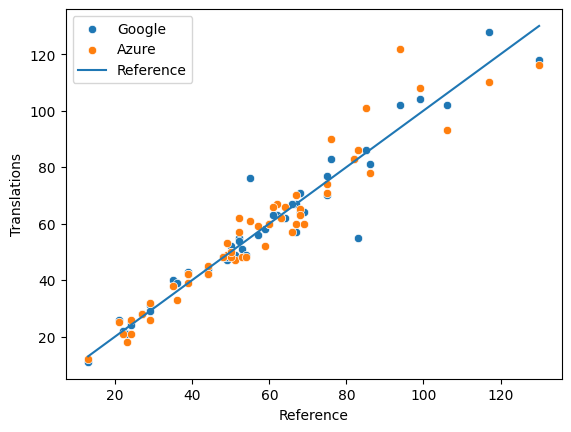
\includegraphics[width=0.8\linewidth]{images/sen_len.png}
    \caption{Length of Sentences}
    \label{fig:sen-len}
\end{figure}

As we can see, the spread of the data points validates our preliminary observation regarding the sentence length. Though this variability is low at shorter lengths, it increases with the increase in length. However, what surprised us the most was that though, we can see that there is a variability in the sentence length, the mean sentence length of the reference, and both the translation systems converge to a common length (see Table \ref{tab:sen-len})

\begin{center}    
\begin{table}[h]
\setlength\extrarowheight{5pt}
\centering
\begin{tabular}{p{4cm}@{}r}
    \textbf{Type} & \textbf{Length} \\
    \hline
    Reference & 57.86 \\
    Google & 57.82 \\
    Azure & 58.0
\end{tabular}
\caption{Mean Sentence Length}
\label{tab:sen-len}
\end{table}
\end{center}

\phantomsection
\section{Automated Metrics \& Human Scores}

Following this we looked at the scores obtained on different metrics, i.e., BLEU, ROUGE, and Human score. We have tabulated our the mean scores obtained for the aforementioned metrics below (see Table \ref{tab:score}).

\begin{center}
    \begin{table}[h]
    \setlength\extrarowheight{10pt}
        \centering
        \begin{tabular}{p{3cm}@{}p{3cm}@{}p{3cm}@{}c}
             & \textbf{Human} & \textbf{BLEU} & \textbf{ROUGE} \\
             \hline
            \textbf{Google} & 87.45 & 84.99 & [84.88, 70.32, 59.86, 79.81] \\
            \textbf{Azure} & 63.53 & 77.6 & [76.38, 56.21, 44.51, 68.22]
 \\ 
        \end{tabular}
        \caption{Mean scores obtained on different metrics}
        \label{tab:score}
    \end{table}
\end{center}

\begin{figure}[h]
    \centering
    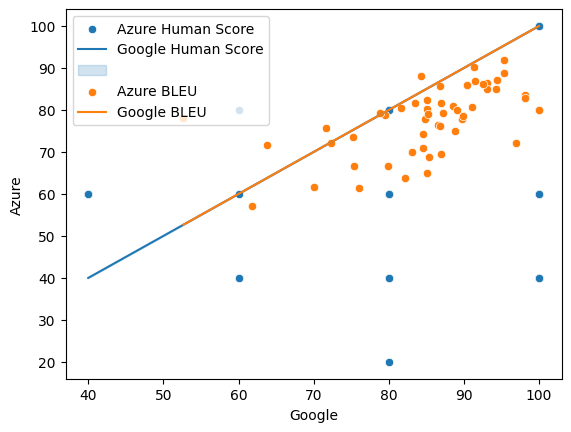
\includegraphics[width=0.9\linewidth]{images/human_bleu.png}
    \caption{Human vs BLEU scores}
    \label{fig:human-v-bleu}
\end{figure}

Table \ref{tab:score} shows a close correlation between the Human score, the BLEU score and the ROUGE-1 score for Google, which is also substantiated by Fig \ref{fig:human-v-bleu}. Even though the Human score is quite different for Azure, it still presents an interpretable picture of both the translation systems. The correlation with Human evaluation validates the BLEU score. BLEU score is usually within the range from 0 to 1, here we have obtained a converted BLEU score in the range of 0 to 100. A higher BLEU score signifies better translation performance. Both Google and Azure translate show a significant improvement when compared to the model Vaswani trained in the paper `\textit{Attention Is All You Need}' \cite{vaswani2017attention} back in 2017, the model had a BLEU score of 41.0.

\begin{figure}[h]
    \centering
    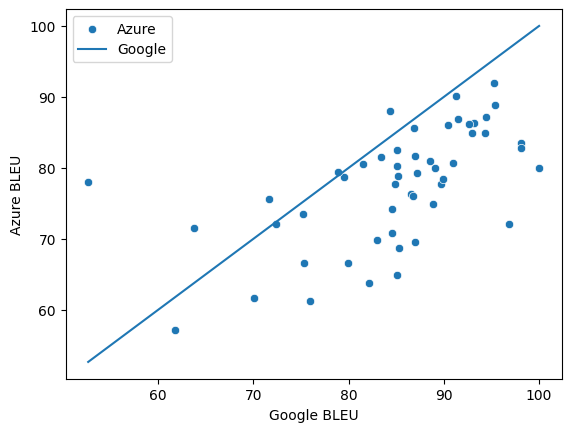
\includegraphics[width=0.9\linewidth]{images/bleu.png}
    \caption{Google vs Azure BLEU score}
    \label{fig:google-v-azure}
\end{figure}

From comparison we also observed that Google Translate performed better than Azure in all of the metrics, the Fig \ref{fig:google-v-azure} visually states the superiority in performance of Google Translate over Azure Translate. There are a few cases where Azure performs better than Google, but Google is the winner overall. This correlation is also supported by the ROUGE metric and the Human score as well Fig \ref{tab:score} Table \ref{tab:score}.

\phantomsection
\section{Manual Analysis}

Now to analyze the translations manually. The fluency of both the systems was remarkable, barely showing any signs of breaking the flow. Though Azure in a couple of cases showed severely improper translations for which the human evaluator assigned it a score of 1 (you can refer to the dataset uploaded online, Section 47, 52, 147, 444 etc.). 

\singlespacing
For Example: \underline{\textbf{Section 444}}
\begin{quote}
    \textbf{English Reference}: `\textit{Lurking house-trespass by night}'\\
    \textbf{Google Translate}: `\textit{Secret house-trespass at night}'\\
    \textbf{Azure Translate}: `\textit{Night Hidden Planet Trespass}'
\end{quote}
\doublespacing

In case of artificiality, there were barely such observations. The most commonly observed divergence were syntactic and lexical divergences, you could find one in almost every sentence. However, the equivalents presented were quite acceptable, except for in some cases. Let's take a look at few examples:-

\singlespacing
\underline{\textbf{Section 47}}
\begin{quote}
    \textbf{English Reference}: `\textit{“Animal”.—The word “animal” denotes any living creature, other than a human being.}'\\
    \textbf{Google Translate}: `\textit{Animal - The word animal denotes any living creature other than human.}'\\
    \textbf{Azure Translate}: `\textit{Fauna : The word animal denotes any living being other than human beings}'
\end{quote}

\underline{\textbf{Section 7}}
\begin{quote}
    \textbf{English Reference}: `\textit{Sense of expression once explained}'\\
    \textbf{Google Translate}: `\textit{Meaning of phrase once explained}'\\
    \textbf{Azure Translate}: `\textit{Meaning of a once clarified phrase}'
\end{quote}

\underline{\textbf{Section 465}}
\begin{quote}
    \textbf{English Reference}: `\textit{Punishment for forgery}'\\
    \textbf{Google Translate}: `\textit{Punishment for forgery}'\\
    \textbf{Azure Translate}: `\textit{Penalty for encryption}'
\end{quote}
\doublespacing

Some of the lexical divergences are acceptable such as in Section 7, while some cause some confusion about the overall meaning of the utterance such as in Section 47. There are cases where there is a bit too much divergence as exemplified by Section 465, where `\textit{forgery}' is replaced by `\textit{encryption}'. There are also cases where these divergences cause the whole meaning of the utterance to be undecipherable, as shown in Section 444 above. There cases of other kinds of divergences as well, Section 7 shows syntactic divergence in case of Azure. Overall, there divergences are in the output of both translation systems. However, in case of Google they are less frequent and mostly acceptable, whereas in case of Azure these divergences are not only frequent but also cause a loss of sense and coherence of the source utterance. The observations seem to correlate with the scores.

\phantomsection
\chapter{Conclusion}

Machine translation has made significant strides since its initial spark was lit by Weaver in 1949. Early rule-based systems have evolved into sophisticated neural machine translation (NMT) models, which leverage vast amounts of data and advanced algorithms to produce translations that are more accurate and fluent. We have traced this very development from just the notion of a Machine Translating text from one language to another, to developing them to the point that their translations astonish us.

The development has gone from the Rule-based systems which relied on predefined linguistic rules and bilingual dictionaries. These systems were limited by their inability to handle linguistic variability and the context-dependent nature of language. This was followed by the Statistical Machine Translation system, which was designed to use large corpora to statistically determine the most likely translations, improving accuracy but still struggling with fluency. Eventually, the advent of NMT in the 2010s revolutionized the field. NMT models use deep learning techniques to capture contextual and syntactic nuances, resulting in more natural and coherent translations. Followed by further progress in the field and the advent of architectures such as `\textit{Transformers}' has allowed these NMT systems to scale and be trained on a large amount of data being able to have extremely long context lengths. Thus not only producing accurate and fluent translation for short-length sentences but whole discourses.

We evaluated the performance of Google Translate and Azure Translate using automated metrics (BLEU and ROUGE) and human evaluations. These assessments provide a comprehensive view of the current state of MT, highlighting both, the aforementioned achievements and ongoing challenges/issues. Let's look at the findings:-

\paragraph{Automated Metrics:}
\begin{itemize}
    \item \textbf{BLEU Scores}: Google Translate achieved a higher BLEU score (84.99) compared to Azure Translate (77.6). This indicates that Google Translate's output aligns more closely with reference translations on average.
    \item \textbf{ROUGE Scores}: Google Translate also outperformed Azure Translate in various ROUGE metrics (ROUGE-1, ROUGE-2, ROUGE-3, and ROUGE-L), reflecting better recall of n-grams and longer phrases from the reference texts
\end{itemize}

\paragraph{Human Evaluation:} Human evaluations offered insights into the fluency, inter-pretability, and overall quality of the translations. Google Translate received a higher human score (87.45) compared to Azure Translate (63.53), indicating superior quality as perceived by human judges.

The manual analysis of translations in line with these metrics and scores, presented us with a clearer picture of the issues which might've produced a lower score, and we also got to understand where and why they produced higher scores. There were quite a few translation divergences. Translation divergences reveal the challenges MT systems face in handling complex linguistic phenomena. These divergences were categorized as syntactic, lexical, and semantic. 

Both systems exhibited issues with maintaining the syntactic structure of the source text. Google Translate handled these divergences more effectively, preserving the original syntax better than Azure Translate. Lexical divergences were quite common. However, Google produced better alternatives, for instance, Google Translate accurately translated ``Punishment for forgery," while Azure Translate's ``Penalty for encryption" was a significant misinterpretation. An example of semantic divergence is the reference translation ``Lurking house-trespass by night,", for which Azure's translation is ``Night Hidden Planet Trespass".

 The comparative analysis highlights that while both Google Translate and Azure Translate have made significant progress, Google Translate consistently outperforms Azure Translate in terms of automated metrics and human evaluations. This can be attributed to Google's advanced NMT models and extensive training data. 

 \paragraph{Google Translate Stengths}
 \begin{itemize}
     \item Higher BLEU and ROUGE scores
     \item Superior human evaluation scores, indicating higher fluency and accuracy
     \item More effective handling of syntactic and lexical divergences
 \end{itemize}

 \paragraph{Azure Translate Weaknesses}
 \begin{itemize}
     \item Lower scores on all metrics compared to Google Translate
     \item More frequent and severe translation errors, particularly in syntax and lexical accuracy
 \end{itemize}

\phantomsection
\section{Suggestions for Further Research}

\begin{itemize}
    \item This analysis could be applied further to general legal texts, such as judgments, court proceedings, or contracts. To better understand its implications in a more general setting.
    \item A bigger dataset could be considered for the same.
    \item Multiple human scorers and different metrics could be considered.
    \item This study could be taken up for other genres, such as literary text, general social media interactions, etc.
\end{itemize}

 The findings underscore the importance of continuous improvement in MT systems, especially for complex texts like the IPC. The superior performance of Google Translate highlights the value of advanced NMT models and extensive training data. Though the performance of these tools is not bad, the limitations observed could create real issues in legal translation and will require human evalua-tion. Overall the comparative analysis of Google Translate and Azure Translate reflects the significant progress in MT over the years. While modern MT tools like Google Translate have achieved remarkable accuracy and fluency, there still remains room for improvement.


\backmatter

\clearpage
\bibliographystyle{apalike}
\phantomsection
\addcontentsline{toc}{chapter}{Bibliography}
\bibliography{ref}

\appendixpage
\clearpage
\appendix
\phantomsection
\addcontentsline{toc}{chapter}{Appendix A}
\chapter*{Appendix A: Codes}

\begin{figure}[h]
    
\includegraphics[width=0.2\linewidth]
    {images/masters_thesis_qr.png}
    \hspace{0.5cm}
    
\includegraphics[width=0.2\linewidth]{images/translating_qr.png}
    \hspace{0.5cm}
    
\includegraphics[width=0.2\linewidth]{images/metrics_qr.png}
    \hspace{0.5cm}
    
\includegraphics[width=0.2\linewidth]{images/analysis_qr.png}
    \caption*{\textbf{A}\hspace{3.3cm}\textbf{B}\hspace{3.3cm}\textbf{C}\hspace{3.3cm}\textbf{D}}
\end{figure}

{\large\textbf{A -}} \href{https://drive.google.com/drive/folders/1TTYZZB0wPYgtiRIskFhZ9-RgWjYXUDtq?usp=sharing}{https://drive.google.com/drive/folders/1TTYZZB0wPYgtiRIskFhZ9-Rg\\WjYXUDtq?usp=sharing} - \textbf{Masters Thesis Main Folder}

{\large\textbf{B -}} \href{https://drive.google.com/drive/folders/1TTYZZB0wPYgtiRIskFhZ9-RgWjYXUDtq?usp=sharing}{https://drive.google.com/drive/folders/1TTYZZB0wPYgtiRIskFhZ9-Rg\\WjYXUDtq?usp=sharing} - \textbf{Translation Notebook}

{\large\textbf{C -}} \href{https://drive.google.com/drive/folders/1TTYZZB0wPYgtiRIskFhZ9-RgWjYXUDtq?usp=sharing}{https://drive.google.com/drive/folders/1TTYZZB0wPYgtiRIskFhZ9-Rg\\WjYXUDtq?usp=sharing} - \textbf{Metrics Calculation Notebook}

{\large\textbf{D -}} \href{https://drive.google.com/drive/folders/1TTYZZB0wPYgtiRIskFhZ9-RgWjYXUDtq?usp=sharing}{https://drive.google.com/drive/folders/1TTYZZB0wPYgtiRIskFhZ9-Rg\\WjYXUDtq?usp=sharing} - \textbf{Analysis Notebook}

\section*{Code for Sampling}

We divided the sample dataset into 50 subsets of 10 and selected a random section out of the 10. Thus having a sample dataset of 51 Sections.

\singlespacing
\begin{minted}{python}
from random import randint

no_of_sections = 510 # Excluding Section 511

sample = [i+randint(1,10) for i in range(0, no_of_sections, 10)]
\end{minted}
\doublespacing

\section*{Code for Translating the Text from Hindi to English, using both Google Translate and Azure Translate}

\singlespacing
\begin{minted}[breaklines]{python}
# Initial Setup

# Importing basic packages which would be required, and mounting the drive to read the dataset and write the output.


from google.colab import drive
import requests, uuid, json
import pandas as pd
drive.mount('/content/drive')

# Reading the dataset into a DataFrame using pandas.

df = pd.read_csv('drive/MyDrive/Masters Thesis - 2019IMSLI003/dataset_IPC.csv')
df.head()

# Google Translate

# Importing required packages for using Google Translate API


from google.cloud import translate_v2 as translate
from google.oauth2 import service_account

# Defining a function for translation using appropriate credentials

def translate_text(text_translate, target_lang='en', credentials_path='drive/MyDrive/careful-ensign-422118-u3-ba712c925224.json'):
  credentials = service_account.Credentials.from_service_account_file(credentials_path)
  translator = translate.Client(credentials=credentials)

  translation = translator.translate(text_translate, target_language=target_lang)

  return translation

# Translating the hindi text using Google Translate and storing it in a column titled 'Google Translate'.

df['Google Translate'] = None

for index,text_to_translate in enumerate(df['Hindi']):
  df.at[index, 'Google Translate'] = translate_text(text_to_translate).get('translatedText')

# Let's take a look at the output.

df.head()

# Azure Cognitive Services Translate

# Setting up the REST API for Azure Translate, including the require key and endpoints, along with other basic attributes.


key = "4ee107e2c5ce40b28c6741d0d0de32a5"
endpoint = "https://api.cognitive.microsofttranslator.com"
location = "centralindia"
path = '/translate'
constructed_url = endpoint + path

params = {
    'api-version': '3.0',
    'from': 'hi',
    'to': ['en']
}

headers = {
    'Ocp-Apim-Subscription-Key': key,
    'Ocp-Apim-Subscription-Region': location,
    'Content-type': 'application/json',
    'X-ClientTraceId': str(uuid.uuid4())
}

# Using Azure Translate to translate and store the text in a column with header 'Azure Translation'.

df['Azure Translate'] = None

for index,text_to_translate in enumerate(df['Hindi']):
  body = [{
    'text': text_to_translate
  }]

  request = requests.post(constructed_url, params=params, headers=headers, json=body)
  response = request.json()

  df.at[index, 'Azure Translate'] = response[0]['translations'][0]['text']

df.head()

# Saving the translated dataset

df.to_csv('drive/MyDrive/Masters Thesis - 2019IMSLI003/dataset_IPC_translated.csv', index=False)
\end{minted}
\doublespacing

\section*{Code to Calculate the Metrics for the Translations}

\singlespacing
\begin{minted}[breaklines]{python}
# Initial Setup

# Connecting Google Drive

from google.colab import drive
drive.mount('/content/drive')

# Importing the basic packages required

import pandas as pd
import re

# Reading the data to be processed into a DataFrame

df = pd.read_csv('drive/MyDrive/Masters Thesis - 2019IMSLI003/dataset_IPC_translated.csv')
df.head()

# Preprocessing

# Making the text lowercase and removing special characters.

def clean(text):
  text = text.lower()
  text = re.sub(r"[^\w]", " ", text)
  text = re.sub(r"\s+", " ", text)
  return text

reference = df['English'].apply(clean)
hypothesis_google = df['Google Translate'].apply(clean)
hypothesis_azure = df['Azure Translate'].apply(clean)

# BLEU

# Importing the required packages and write a function to calculate the BLEU score (sentence BLEU in this case)


import math
from nltk.translate.bleu_score import sentence_bleu

def calculate_bleu_score(reference, hypothesis, weights=(0.25, 0.25, 0.25, 0.25)):
  if not reference or not hypothesis:
    return None

  if isinstance(reference, str):
    reference = [reference]

  try:
    bleu_score = sentence_bleu(reference, hypothesis, weights=weights, smoothing_function=None)
  except ZeroDivisionError:
    bleu_score = None

  return bleu_score

# Calculating the BLEU metric for the dataset and adding it to the DataFrame. We also calculate the token length of each section, for reference as we translated counterparts.

df['reference_len'] = None
df['google_len'] = None
df['azure_len'] = None
df['google_bleu'] = None
df['azure_bleu'] = None

for index, refrence, google_hypothesis, azure_hypothesis in zip(range(len(df)), reference, hypothesis_google, hypothesis_azure):
  google_bleu = calculate_bleu_score(refrence, google_hypothesis)
  azure_bleu = calculate_bleu_score(refrence, azure_hypothesis)

  df.at[index, 'reference_len'] = len(refrence.split())
  df.at[index, 'google_len'] = len(google_hypothesis.split())
  df.at[index, 'azure_len'] = len(azure_hypothesis.split())

  df.at[index, 'google_bleu'] = round(google_bleu*100, 2)
  df.at[index, 'azure_bleu'] = round(azure_bleu*100, 2)

# ROGUE

# Importing the required packages and calculating ROGUE metric, and defining a function to calculate the ROUGE score.


from rouge_score import rouge_scorer

rouge_metrics = ['rouge1', 'rouge2', 'rouge3', 'rougeL']
scorer = rouge_scorer.RougeScorer(rouge_metrics)

def calculate_rouge_score(reference, hypothesis):
  if not reference or not hypothesis:
    return None

  scores = scorer.score(hypothesis, reference)

  scores_f = [round(scores[i][2]*100,2) for i in rouge_metrics]
  return scores_f

# Calculating the ROUGE score for the dataset.

df['google_rouge'] = None
df['azure_rouge'] = None

for index, hypothesis, google_hypothesis, azure_hypothesis in zip(range(len(df)), reference, hypothesis_google, hypothesis_azure):
  google_rouge = calculate_rouge_score(hypothesis, google_hypothesis)
  azure_rouge = calculate_rouge_score(hypothesis, azure_hypothesis)
  df.at[index, 'google_rouge'] = google_rouge
  df.at[index, 'azure_rouge'] = azure_rouge

# Writing the calculated metrics to csv

df.to_csv('drive/MyDrive/Masters Thesis - 2019IMSLI003/dataset_IPC_metrics.csv', index=False)
\end{minted}
\doublespacing
\clearpage
\appendix
\phantomsection
\addcontentsline{toc}{chapter}{Appendix B}
\chapter*{Appendix B: Tables}

There are 51 entries for each of the sections mentioned below, which would take quite a number of pages to be printed, due to that reason we have tabulated the first 5 entries from each section, and have attached a link to the whole dataset, uploaded to the Google Drive (just like the notebooks) for future reference.

Link for the Dataset: \href{https://drive.google.com/drive/folders/1bzr7zFtRo2lOGgZHOYy6GC69jYzhsx8n?usp=drive_link}{https://drive.google.com/drive/folders/1bzr7zFtRo2lOG\\gZHOYy6GC69jYzhsx8n?usp=drive\_link}

\begin{figure}[h]
    \centering
    
\includegraphics[width=0.2\linewidth]{images/data_sheets_qr.png}
\end{figure}

\singlespacing
\section*{Sampled Dataset}
\begin{longtable}{|c|p{6cm}|p{6cm}|}
\hline
\textbf{Section} & \textbf{English} & \textbf{Hindi} \\
\hline
7 & Sense of expression once explained.—Every expression which is explained in any part of this Code, is used in every part of this Code in conformity with the explanation. & {\hindifont एक बार स्पष्टीकॄत वाक्यांश का अभिप्राय - हर वाक्यांश, जिसका स्पष्टीकरण इस संहिता के किसी भाग में किया गया है, इस संहिता के हर भाग में उस स्पष्टीकरण के अनुरूप ही प्रयोग किया गया है।} \\
\hline
19 & “Judge”.—The word “Judge” denotes not only every person who is officially designated as a Judge, but also every person who is empowered by law to give, in any legal proceeding, civil or criminal, a definitive judgment, or a judgment which, if not appealed against, would be definitive, or a judgment which, if confirmed by some other authority, would be definitive, or who is one of a body or persons, which body of persons is empowered by law to give such a judgment. & {\hindifont न्यायाधीश - न्यायाधीश शब्द न केवल हर ऐसे व्यक्ति का द्योतक है, जो पद रूप से न्यायाधीश अभिहित हो, किन्तु उस हर व्यक्ति का भी द्योतक है, जो किसी क़ानूनी कार्यवाही में, चाहे वह सिविल हो या आपराधिक, अन्तिम निर्णय या ऐसा निर्णय, जो उसके विरुद्ध अपील न होने पर अन्तिम हो जाए या ऐसा निर्णय, जो किसी अन्य प्राधिकारी द्वारा पुष्ट किए जाने पर अन्तिम हो जाए, देने के लिए विधि द्वारा सशक्त किया गया हो, अथवा जो उस व्यक्ति निकाय में से एक हो, जो व्यक्ति निकाय ऐसा निर्णय देने के लिए विधि द्वारा सशक्त किया गया हो।} \\
\hline
25 & “Fraudulently”.—A person is said to do a thing fraudulently if he does that thing with intent to defraud but not otherwise. & {\hindifont कपटपूर्वक - कोई व्यक्ति किसी कार्य को कपट करने के आशय से करता है, उसे कपटपूर्वक कृत्य कहा जाता है, अन्यथा नहीं।} \\
\hline
37 & Co-operation by doing one of several acts constituting an offence.—When an offence is committed by means of several acts, whoever intentionally co-operates in the commission of that offence by doing any one of those acts, either singly or jointly with any other person, commits that offence. & {\hindifont कई कार्यों में से किसी एक कार्य को करके अपराध गठित करने में सहयोग करना। - जब कि कोई अपराध कई कार्यों द्वारा किया जाता है, तब जो भी कोई या तो अकेले या किसी अन्य व्यक्ति के साथ सम्मिलित होकर उन कार्यों में से कोई एक कार्य करके उस अपराध के किए जाने में साशय सहयोग करता है, तो वह उस अपराध को करता है।} \\
\hline
47 & “Animal”.—The word “animal” denotes any living creature, other than a human being. & {\hindifont जीवजन्तु - जीवजन्तु शब्द मानव से भिन्न किसी जीवधारी का द्योतक है ।} \\
\hline
\end{longtable}
\doublespacing

\section*{Translated Sample}

\singlespacing
\begin{tabular}{|c|p{6cm}|p{6cm}|}
\hline
\textbf{Section} & \textbf{Google Translate} & \textbf{Azure Translate} \\
\hline
7 & Meaning of a once clarified phrase - Every phrase which is explained in any part of this Code is used in every part of this Code in the same manner as that explanation. & Meaning of a once clarified phrase - Every phrase which is explained in any part of this Code is used in every part of this Code in the same manner as that explanation. \\
\hline
19 & Judge.—The word `Judge' denotes not only every person who is designated a judge by office, but also of every person  Who has been empowered by law to give a final judgment in any legal proceeding, whether civil or criminal, or a decision which becomes final when there is no appeal against it or a decision which becomes final when confirmed by any other authority, or who is one of the body of persons; A body of persons empowered by law to give such a decision. & The word `Judge' denotes not only every person who is designated a judge by office, but also every person who is empowered by law to give a final judgment in any legal proceeding, whether civil or criminal, or a decision which becomes final when there is no appeal against it or a decision which becomes final when confirmed by any other authority, or who is one of a body of persons empowered by law to give such a decision.  \\
\hline
25 & Fraudulently – A person does something with the intention of deceit, it is said to be an act of deception, not otherwise. & Fraudulently - When a person does something with the intent to deceive, it is said to be a fraudulent act and not otherwise. \\
\hline
37 & To cooperate in constituting an offense by doing any one of several tasks. - When an offense is committed by several acts, whoever intentionally cooperates in the commission of that offense by either alone or in association with any other person by doing any of those acts, commits that offense. & To cooperate in committing an offense by doing any one of several acts. - When an offense is committed by several acts, whoever intentionally cooperates in the commission of that offense by doing any one of those acts, either alone or in association with any other person, commits that offense. \\
\hline
47 & Fauna : The word animal denotes any living being other than human beings. & Animal - The word animal denotes any living creature other than a human being. \\
\hline
\end{tabular}

\section*{Metrics \& Scores}

\vspace{0.5cm}

\subsection*{Sentence Length \& BLEU Score}

\begin{center}
    \begin{table}[h]
    \setlength\extrarowheight{5pt}
    \centering
    \begin{tabular}{|c|c|c|c|c|c|}
        \hline
        \textbf{Section} & \textbf{reference\_len} & \textbf{google\_len} & \textbf{azure\_len} & \textbf{google\_bleu} & \textbf{azure\_bleu} \\
        \hline
        7 & 29 & 31 & 32 & 72.36 & 72.13 \\
        \hline
        19 & 83 & 55 & 86 & 52.68 & 78.06 \\
        \hline
        25 & 22 & 22 & 21 & 75.99 & 61.3 \\
        \hline
        37 & 49 & 47 & 49 & 84.35 & 87.98 \\
        \hline
        47 & 13 & 11 & 12 & 86.59 & 76.39 \\
        \hline
    \end{tabular}
\end{table}
\end{center}

\subsection*{ROUGE Score}

\begin{center}
    \begin{table}[h]
    \setlength\extrarowheight{5pt}
    \centering
    \begin{tabular}{|c|c|c|}
        \hline
        \textbf{Section} & \textbf{google\_rouge} & \textbf{azure\_rouge}\\
        \hline
        7 & [73.33, 51.72, 42.86, 73.33] & [75.41, 57.63, 56.14, 75.41] \\
        \hline
        19 & [73.91, 57.35, 47.76, 69.57] & [74.56, 47.9, 30.3, 69.82] \\
        \hline
        25 & [63.64, 28.57, 10.0, 45.45] & [46.51, 24.39, 10.26, 37.21] \\
        \hline
        37 & [83.33, 61.7, 52.17, 70.83] & [79.59, 60.42, 44.68, 63.27] \\
        \hline
        47 & [91.67, 81.82, 80.0, 91.67] & [80.0, 52.17, 38.1, 72.0] \\
        \hline
    \end{tabular}
\end{table}
\end{center}

\subsection*{Human Assigned Scores}

\begin{table}[h]
    \setlength\extrarowheight{5pt}
    \centering
    \begin{tabular}{|c|c|c|}
        \hline
        \textbf{Section} & \textbf{google\_hum\_score} & \textbf{azure\_hum\_score} \\
        \hline
        7 & 4 & 4 \\
        \hline
        19 & 3 & 3 \\
        \hline
        25 & 4 & 2 \\
        \hline
        37 & 4 & 3 \\
        \hline
        47 & 5 & 2 \\
        \hline
    \end{tabular}
\end{table}

\clearpage
\appendix

\newpage
\thispagestyle{empty}

\centering
{\section*{The Tex source code, dataset, and Jupyter notebooks have also been uploaded to Github}

\vspace{5cm}

\begin{figure}[h]
    \centering
    
\includegraphics[width=0.5\textwidth]{images/qr_github.png}
\end{figure}

\vspace{5cm}

\Large\textbf{Link:}\href{https://github.com/two048/masters-thesis}{https://github.com/two048/masters-thesis}}

\end{document}